\begin{savequote}[45mm]
\ascii{Any fool can write code that a computer can understand. Good programmers write code that humans can understand.}
\qauthor{\ascii{- Martin Flower}}
\end{savequote}

\chapter{编程环境} 
\label{ch:prog-env}

\begin{content}

为了实现\tf{}的快速入门,本章将介绍\tf{}的编程环境,包括代码结构,工程构建,环境验证,以便对\tf{}有一个基本的感性认识。

\end{content}

\section{代码结构}

\begin{content}

\subsection{克隆源码}

首先,从\ascii{Github}上克隆\tf{}的源代码。


\begin{leftbar}
\begin{python}
$ git clone git@github.com:tensorflow/tensorflow.git
\end{python}
\end{leftbar}

然后,切换到最新的稳定分支上。例如,\code{r1.2}分支。

\begin{leftbar}
\begin{python}
$ cd tensorflow
$ git checkout r1.2
\end{python}
\end{leftbar}

\subsection{源码结构}

可以运行如下命令,打印出\tf{}源码的组织结构。

\begin{leftbar}
\begin{python}[]
$ tree -d -L 1 ./tensorflow
\end{python}
\end{leftbar}

其中,本书将重点关注\code{core, python, c}组件,部分涉及\code{cc, stream\_executor}组件。

\begin{leftbar}
\begin{c++}[caption={TensorFlow源码结构}]
./tensorflow
├── c
├── cc
├── compiler
├── contrib
├── core
├── docs_src
├── examples
├── g3doc
├── go
├── java
├── python
├── stream_executor
├── tools
└── user_ops
\end{c++}
\end{leftbar}

如果在\ascii{Mac OS}下,可以运行\code{cloc}统计\tf{}的代码行,截止当前最新版本\code{1.3},\tf{}拥有大约\ascii{100}万代码;其中,\ascii{53}万行\ascii{C/C++}代码,\ascii{37}万行\ascii{Python}代码。因此,可以推测\tf{}的\ascii{Python}的编程接口是最完善的,相比其他编程语言还处于起步阶段。

\begin{leftbar}
\begin{python}[caption={TensorFlow代码统计}]
-------------------------------------------------------
Language             files    blank    comment    code
-------------------------------------------------------
C++                   2238    77610     68275    443099
Python                1881    92018    151807    369399
C/C++ Header          1175    27392     46215     86691
Markdown               218     8859         2     30925
CMake                   50     2183       986     16398
Go                      28     1779     13290     15003
Java                    72     1789      3111      7779
Bourne Shell           103     1487      3105      6074
Protocol Buffers        87     1313      3339      3452
Objective C++            9      227       181      1201
C                        8      157       130       941
make                     4      105       136       612
XML                     25      135       265       315
Groovy                   3       46        74       246
Maven                    5       21         4       245
DOS Batch                9       30         0       143
Dockerfile               7       41        69       133
Perl                     2       29        38       130
Bourne Again Shell       3       24        63       111
JSON                     3        0         0        23
Objective C              1       10        13        21
YAML                     1        3        24        15
-------------------------------------------------------
SUM:                  5932   215258    291127    982956
-------------------------------------------------------
\end{python}
\end{leftbar}

\subsection{Core}

内核的源码物理组织如下所示,主要包括平台,实用函数库,基础框架,\ascii{Protobuf}定义,本地运行时,分布式运行时,图操作,\ascii{OP}定义,以及\ascii{Kernel}实现等组成,这是本书重点剖析的对象。

\begin{leftbar}
\begin{c++}[caption={Core源码结构}]
./tensorflow/core
├── common_runtime
├── debug
├── distributed_runtime
├── example
├── framework
├── graph
├── grappler
├── kernels
├── lib
├── ops
├── platform
├── profiler
├── protobuf
├── public
├── user_ops
└── util
\end{c++}
\end{leftbar}

其中,\code{core}主要由\code{C++}实现,大约有\ascii{26}行代码。

\begin{leftbar}
\begin{python}[caption={Core代码统计}]
-------------------------------------------------------
Language             files    blank   comment      code
-------------------------------------------------------
C++                   1368    44791     38968    259289
C/C++ Header           653    15040     24474     50506
Protocol Buffers        57      736      2371      1806
Markdown                11      327         0      1285
JSON                     2        0         0        18
-------------------------------------------------------
SUM:                  2091    60894     65813    312904
-------------------------------------------------------
\end{python}
\end{leftbar}

\subsection{Python}

\ascii{Python}定义和实现了\tf{}的编程模型,并对外开放\ascii{API}供程序员使用,其源码物理组织如下所示,这也是本书重点剖析的对象。

\begin{leftbar}
\begin{c++}[caption={Python源码结构}]
./tensorflow/python
├── client
├── debug
├── estimator
├── feature_column
├── framework
├── grappler
├── kernel_tests
├── layers
├── lib
├── ops
├── platform
├── profiler
├── saved_model
├── summary
├── tools
├── training
├── user_ops
└── util
\end{c++}
\end{leftbar}

其中,\code{core}主要由\code{C++}实现,大约有\ascii{26}行代码。

\begin{leftbar}
\begin{python}[caption={Python代码统计}]
-------------------------------------------------------
Language            files     blank   comment      code
-------------------------------------------------------
Python                714     45769     69407    179565
C++                    20       496       506      3658
C/C++ Header           15       207       387       363
Markdown                4        48         0       200
Protocol Buffers        3        16        10        71
Bourne Shell            1        13        28        68
-------------------------------------------------------
SUM:                  757     46549     70338    183925
-------------------------------------------------------
\end{python}
\end{leftbar}

\subsection{Contrib}

\code{contrib}是第三方贡献的编程库,它也是\tf{}标准化之前的实验性编程接口。犹如\ascii{Boost}社区与\ascii{C++}标准之间的关系。当\code{contrib}的接口成熟后,便会被\tf{}标准化,并从\code{contrib}中搬迁至\code{core, python}中,并正式对外发布\ascii{API}。

\begin{leftbar}
\begin{python}[caption={Contrib源码结构}]
./tensorflow/contrib
├── android
├── batching
├── bayesflow
├── benchmark_tools
├── boosted_trees
├── cloud
├── cluster_resolver
├── cmake
├── compiler
├── copy_graph
├── crf
├── cudnn_rnn
├── data
├── decision_trees
├── deprecated
├── distributions
├── eager
├── factorization
├── ffmpeg
├── framework
├── fused_conv
├── gdr
├── graph_editor
├── grid_rnn
├── hooks
├── hvx
├── image
├── imperative
├── input_pipeline
├── integrate
├── keras
├── kernel_methods
├── labeled_tensor
├── layers
├── learn
├── legacy_seq2seq
├── linalg
├── linear_optimizer
├── lookup
├── losses
├── makefile
├── memory_stats
├── meta_graph_transform
├── metrics
├── mpi
├── nccl
├── ndlstm
├── nearest_neighbor
├── nn
├── opt
├── pi_examples
├── predictor
├── quantization
├── reduce_slice_ops
├── remote_fused_graph
├── resampler
├── rnn
├── saved_model
├── seq2seq
├── session_bundle
├── signal
├── slim
├── solvers
├── sparsemax
├── specs
├── staging
├── stat_summarizer
├── stateless
├── tensor_forest
├── tensorboard
├── testing
├── text
├── tfprof
├── timeseries
├── tpu
├── training
├── util
├── verbs
└── xla_tf_graph
\end{python}
\end{leftbar}

由于\tf{}社区相当活跃,\code{contrib}的变更相当频繁,截止\ascii{1.3}版本,大约有\ascii{23}万行代码,主要由\ascii{Python}设计编程接口,部分运行时由\ascii{C++}实现。

\begin{leftbar}
\begin{python}[caption={Contrib代码统计}]
-------------------------------------------------------
Language            files     blank   comment      code
-------------------------------------------------------
Python               1007     41436     75096    170355
C++                   201      5500      5313     32944
CMake                  48      2172       955     16358
C/C++ Header           99      1875      2867      6583
Markdown               46      1108         0      3485
Bourne Shell           18       232       386      1272
C                       7       151       118       931
Protocol Buffers       20       224       454       680
make                    4       105       136       612
Java                    2        77       209       335
Groovy                  1        10        20        75
Bourne Again Shell      1         6        15        59
Dockerfile              1         2         1        14
XML                     2         3         0         9
-------------------------------------------------------
SUM:                 1457     52901     85570    233712
-------------------------------------------------------
\end{python}
\end{leftbar}

\subsection{StreamExecutor}

\ascii{StreamExecutor}是\ascii{Google}另一个开源组件库,它提供了主机端(\ascii{host-side})的编程模型和运行时环境,实现了对\ascii{CUDA}和\ascii{OpenCL}的统一封装。使得主机端的代码中,可以将功能相同、数据并行的内核函数无缝地部署在\code{CUDA}或\code{OpenCL}的计算设备上执行。

目前,\ascii{StreamExecutor}被大量应用于\ascii{Google}内部的\ascii{GPGPU}应用程序的运行时。其中,\tf{}运行时也包含了一个\ascii{StreamExecutor}的快照版本,用于封装\ascii{CUDA}和\code{OpenCL}的运行时,本书将详细介绍其系统架构与工作原理。

\begin{leftbar}
\begin{c++}[caption={StreamExecutor源码结构}]
./tensorflow/stream_executor
├── cuda
├── host
├── lib
└── platform
\end{c++}
\end{leftbar}

其中,\ascii{StreamExecutor}使用\code{C++}实现,大约有\ascii{2.5}万行代码。

\begin{leftbar}
\begin{python}[caption={StreamExecutor代码统计}]
-------------------------------------------------------
Language            files     blank   comment      code
-------------------------------------------------------
C++                    43      2440      1196     16577
C/C++ Header           81      2322      5080      8625
-------------------------------------------------------
SUM:                  124      4762      6276     25202
-------------------------------------------------------
\end{python}
\end{leftbar}

\subsection{Compiler}

灵活性是\tf{}最重要的设计目标和核心优势,因此\tf{}的系统架构具有良好的可扩展性,\tf{}可用于定义任意图结构,并使用异构的计算设备有效地执行。但是,熊掌与鱼翅不可兼得,当低级\code{OP}组合为计算子图时,并期望在\code{GPU}上有效执行时,运行时将启动多个\code{Kernel}的运算,其速度更加缓慢。

因此,\tf{}分解和组合\code{OP}的方法,在运行时并不能保证以最有效的方式运行。此时,\ascii{XLA}技术孕育而生,它使用\ascii{JIT}编译技术来分析运行时的计算图,它将多个\code{OP}融合在一起,并生成更高效的本地机器代码。

\begin{leftbar}
\begin{python}[caption={Compiler源码结构}]
./tensorflow/compiler
├── aot
├── jit
├── plugin
├── tests
├── tf2xla
└── xla
\end{python}
\end{leftbar}

\ascii{XLA}技术目前处于前期研发阶段,是\tf{}社区较为活跃研究方向,代码规模大约为\ascii{12.5}万行。

\begin{leftbar}
\begin{python}[caption={Compiler代码统计}]
-------------------------------------------------------
Language            files     blank   comment      code
-------------------------------------------------------
C++                   455     19010     18334    102537
C/C++ Header          250      5939     10323     15510
Python                 37      1255      1416      6446
Protocol Buffers        5       312       501       781
Markdown                2         0         0         3
-------------------------------------------------------
SUM:                  749     26516     30574    125277
-------------------------------------------------------
\end{python}
\end{leftbar}

\end{content}

\section{工程构建}

\begin{content}

通过\tf{}源码构建过程,了解\tf{}所依赖的构建方式、工具,及其依赖的组件库、及其第三方工具包,以便初步建立对\tf{}的感性认识。但因篇幅受限,本节仅以\ascii{Mac OS}为例,讲述\tf{}的源码编译、安装、及其验证过程。其他操作系统,及其\ascii{CUDA}环境安装,请查阅\tf{}官方文档。

\subsection{环境准备}

在构建\ascii{TensorFlow}前,需要事先准备构建环境。\ascii{TensorFlow}的前端是一个支持多语言的编程接口,后端是一个使用\ascii{C++}实现的执行系统。因此,编译\ascii{TensorFlow}源代码之前,需要事先安装前端系统所使用编程语言的编译器、解释器、及其运行时环境。例如,使用\ascii{Python}作为编程接口,需要事先安装\ascii{Python2},或者\ascii{Python3}。下文以\ascii{Python2}为例,讲述环境准备过程;如果使用\ascii{Python3},请查阅相关文档。

其次,也需要事先安装\ascii{GCC, Clang}等\ascii{C++}的编译器,用于编译后端系统实现。本文将不再冗述这两个方面的环境安装过程。另外,\ascii{TensorFlow}使用\ascii{Bazel}的构建工具。因此,需要事先安装\ascii{Bazel}。不幸的是,因为\ascii{Bazel}依赖于\ascii{JDK},因此在安装\ascii{Bazel}之需要前先安装\ascii{JDK}。

\subsubsection{安装JDK}

可以从\ascii{Oracle}官网上下载至少\ascii{1.8}及以上版本的\ascii{JDK},然后配置相关环境变量。

\begin{leftbar}
\begin{python}
$ sudo mkdir -p /usr/lib/jvm
$ sudo tar zxvf jdk-8u51-linux-x64.tar.gz -C /usr/lib/jvm
$ sudo ln -s /usr/java/jdk1.8.0_51 /usr/java/default
\end{python}
\end{leftbar}

创建\ascii{Java}相关环境变量,并添加到\code{~/.bashrc}配置文件中。

\begin{leftbar}
\begin{python}
$ echo 'export JAVA_HOME=/usr/java/default' >> ~/.bashrc
$ echo 'export PATH="$JAVA_HOME/bin:$PATH"' >> ~/.bashrc
\end{python}
\end{leftbar}

\subsubsection{安装Bazel}

在\ascii{Mac OS}上,可以使用\ascii{brew}安装\ascii{Bazel}。

\begin{leftbar}
\begin{python}
$ brew install bazel
\end{python}
\end{leftbar}

如果系统未安装\ascii{brew},可以执行如下命令先安装\ascii{brew}。当然,需要事先安装\ascii{Ruby}解释器,在此不再冗述。

\begin{leftbar}
\begin{python}
$ /usr/bin/ruby -e "$(curl -fsSL https://raw.githubusercontent.com/Homebrew/install/master/install)"
\end{python}
\end{leftbar}

\subsubsection{安装Swig}

\ascii{TensorFlow}使用\ascii{Swig}构建多语言编程的环境,因此需要事先安装\ascii{Swig}工具包。

\begin{leftbar}
\begin{python}
$ brew install swig
\end{python}
\end{leftbar}

\subsubsection{安装Python依赖包}

使用\ascii{pip}安装\ascii{TensorFlow}所依赖的\ascii{Python}包。

\begin{leftbar}
\begin{python}
$ sudo pip install six numpy wheel
\end{python}
\end{leftbar}

如果系统未安装\ascii{pip},则可以使用\ascii{brew}先安装\ascii{pip}:

\begin{leftbar}
\begin{python}
$ brew install pip
\end{python}
\end{leftbar}

\subsection{配置}

编译环境准备就绪之后,便可以执行\code{./configure}配置\ascii{TensorFlow}的编译环境了。特殊地,当系统不支持\ascii{GPU},则可以不需要配置和安装\ascii{CUDA},及其\ascii{cuDNN}。

\begin{leftbar}
\begin{python}
$ ./configure
\end{python}
\end{leftbar}

\subsection{构建}

当配置成功后,使用\ascii{Bazel}启动\ascii{TensorFlow}的编译。特殊地,当需要支持\ascii{GPU}时,添加\code{--config=cuda}编译选项。

\begin{leftbar}
\begin{python}
$ bazel build --config=opt //tensorflow/tools/pip_package:build_pip_package
\end{python}
\end{leftbar}

编译成功后,便可以构建\ascii{TensorFlow}的\ascii{Wheel}包。

\begin{leftbar}
\begin{python}
$ bazel-bin/tensorflow/tools/pip_package/build_pip_package /tmp/tensorflow_pkg
\end{python}
\end{leftbar}

\subsection{安装}

当\ascii{Whell}包构建成功后,便可以使用\ascii{pip}安装\ascii{TensorFlow}了。

\begin{leftbar}
\begin{python}
$ sudo pip install /tmp/tensorflow_pkg/tensorflow-1.2.0-py2-none-any.whl
\end{python}
\end{leftbar}

\subsection{验证}

启动\ascii{Python}解释器,验证\ascii{TensorFlow}安装是否成功。

\begin{leftbar}
\begin{python}
$ python
>>> import tensorflow as tf
>>> hello = tf.constant('Hello, TensorFlow!')
>>> sess = tf.Session()
>>> print(sess.run(hello))
Hello, TensorFlow!
\end{python}
\end{leftbar}

\end{content}

\section{技术栈}

\begin{content}

如\refig{tf-stack}所示,按照系统的层次结构展示了\tf{}的技术栈,构成了\tf{}生态系统的核心。

\begin{figure}[!htbp]
\centering
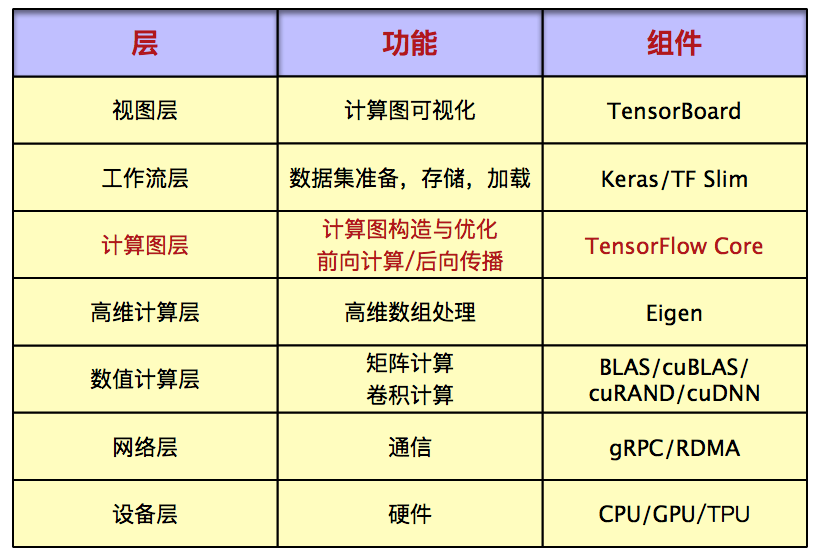
\includegraphics[width=0.7\textwidth]{figures/tf-stack.png}
\caption{TensorFlow技术栈}}
 \label{fig:tf-stack}
\end{figure}

\end{content}
